\section{Processi Primari}
\subsection{Fornitura}
\subsubsection{Scopo}
Lo scopo del processo\textsuperscript{G} di fornitura, come definito nello standard ISO/IEC/IEEE 12207:1995, è di determinare quali strumenti, risorse e competenze siano necessarie per lo svolgimento del progetto. 

\subsubsection{Descrizione}
La presente sezione contiene tutte le norme che ogni membro del gruppo è tenuto a seguire, durante le varie fasi di svolgimento del progetto, per poter divenire fornitori\textsuperscript{G} del proponente\textsuperscript{G} zero12 e dei committenti\textsuperscript{G} Prof. Tullio Vardanega e Prof. Riccardo Cardin. 
Verrà definita la gestione dei rapporti con il proponente, comprese consegna e manutenzione del prodotto finale.

\subsubsection{Rapporti con il proponente}
Il gruppo entrerà in contatto con il proponente zero12 per:
\begin{itemize}
	\item Approfondire aspetti chiave con il proponente per far fronte ai sui bisogni; 
	\item Chiarire ogni eventuale dubbio emerso;
	\item Stimare tempistiche di lavoro;
	\item Individuare le strategie lavorative più efficaci;
	\item Definizione dei requisiti e vincoli da rispettare;
	\item Proporre nuove soluzioni o alternative, discutendo di vantaggi, svantaggi e fattibilità.
\end{itemize}
A meno di accordi diversi con il proponente non sarà prevista nessuna manutenzione futura del prodotto dopo l'avvenuta consegna e collaudo.

\subsubsection{Materiale fornito}
Il materiale che il gruppo fornirà al proponente e ai committenti sono:
\begin{itemize}
  \item \textbf{\AdR} contiene l’analisi dei casi d’uso e dei requisiti con lo scopo di: 
	\begin{itemize}
		\item Determinare tutte e sole le funzionalità che saranno offerte dal prodotto finale;
		\item Chiarire ogni ambiguità che potrebbe sorgere nella comprensione del capitolato.
	\end{itemize}  

  \item \textbf{\PdP} contiene la pianificazione preventiva dei tempi, l’analisi dei rischi, il consuntivo di periodo, la data di consegna e i costi previsti;

  \item \textbf{\PdQ} contiene le modalità adottate in verifica e validazione, assicurando che la qualità dei processi e dei prodotti rispetti le aspettative.
  
  \item \textit{\textbf{Proof of Concept}} piccolo software di esempio che servirà al gruppo per determinare la fattibilità pratica e dimostrare la fondatezza e applicabilità di concetti fondamentali e costituenti in relazione al prodotto finale. 

\end{itemize}

\subsection{Sviluppo}
\subsubsection{Scopo}
Lo scopo del processo di sviluppo, secondo lo standard  ISO/IEC/IEEE 12207:1995 è definire compiti e attività da eseguire per realizzare il prodotto finale richiesto dal proponente.
\subsubsection{Descrizione}
Sono elencate e dopo trattate le seguenti attività di questo processo:
\begin{itemize}
  \item Analisi dei requisiti;
  \item Progettazione;
  \item Codifica.
\end{itemize}
\subsubsection{Analisi dei requisiti}
\paragraph{Scopo}
\'E compito di ogni \textit{Analista} scrivere il documento di \textit{Analisi dei Requisiti}. Lo scopo di tale documento è:
\begin{itemize}
  \item aiutare i \textit{Progettisti};
  \item stabilire ciò che si è concordato con il cliente;
  \item fornire una base per chiunque prenda sottomano il prodotto per miglioramenti;
  \item aiutare le revisioni del codice;
  \item fornire riferimenti utili ai \textit{Verificatori};
  \item tracciare il lavoro per stimarne i costi.
\end{itemize}

\paragraph{Descrizione}
L’obiettivo è la realizzazione dell’architettura del sistema.

\paragraph{Struttura}
La struttura potrà essere soggetta a cambiamenti. Attualmente, \AdR presenta questa struttura:
\begin{itemize}
  \item Introduzione al documento;
  \item Descrizione generale, dove sono presenti requisiti estrapolati sia dal capitolato d’appalto che dagli incontri effettuati con il proponente (verbali esterni);
  \item Casi d'uso relativi alle varie funzionalità fruibili nella piattaforma\textsuperscript{G};
  \item Requisiti che dovrà soddisfare la piattaforma.
\end{itemize}

\paragraph{Classificazione casi d'uso}
La struttura adottata per la classificazione dei casi d'uso è la seguente: \\
\centerline{\textbf{UC[Identificatore][CodiceCasoBase](.[CodiceSottoCaso])*}}
Composta da:
\begin{itemize}
\item \textbf{UC}: acronimo di "Use Case";
\item \textbf{Identificatore}: che può assumere le diverse espressioni letterali:
	\begin{itemize}
		\item \textbf{W}: identifica un caso d'uso relativo alla WebApp;
		\item \textbf{E}: identifica un caso d'uso d'errore.
	\end{itemize}
\item \textbf{CodiceCasoBase}: ID del caso d'uso generico;
\item \textbf{CodiceSottoCaso}: ID opzionale per i sottocasi di un caso d'uso.
\end{itemize}

Ogni caso d'uso è descritto da: 
\begin{itemize}
    \item \textbf{Id}: codice identificativo del caso d'uso, stabilito come enunciato sopra;
    \item \textbf{Nome}: stringa titolo del caso d'uso posta dopo l'id;
    \item \textbf{Diagramma UML}: diagramma per rappresentare graficamente il caso d'uso;
    \item \textbf{Descrizione}: breve descrizione del caso d'uso;
    \item \textbf{Attori}: entità esterne al sistema che interagiscono con esso. Ne esistono due varianti : 
    \begin{itemize}
    \item \textbf{Primario}: interagisce con il sistema per raggiungere un obiettivo;
    \item \textbf{Secondario}: aiuta il primario a raggiungere l'obiettivo. Non utilizzato.
    \end{itemize}
    \item \textbf{Precondizione}: descrive lo stato del sistema prima del verificarsi del caso d'uso;
    \item \textbf{Postcondizione}: descrive lo stato del sistema dopo che si è verificato il caso d'uso;
    \item \textbf{Scenario principale}: elenco numerato che descrive il flusso degli eventi del caso d'uso;
    \item \textbf{Scenario secondario/alternativo} : elenco numerato che descrive il flusso degli eventi del caso d'uso dopo un evento imprevisto che lo ha deviato dal caso principale. Può non esserci o possono esserci più di uno;
    \item \textbf{Estensioni}: utilizzate nei scenari alternativi. Se si verifica una determinata situazione, il caso d'uso collegato all'estensione viene interrotto.
\end{itemize}

\paragraph{Modello di Diagramma di un Caso D'Uso}

Qui di seguito viene mostrato un esempio di diagramma di un caso d'uso con tutte le componenti UML usate.
\begin{figure}[!h]
\centering
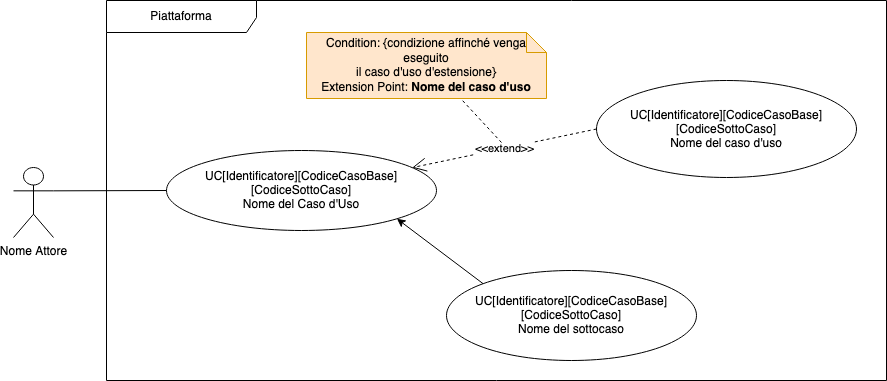
\includegraphics[scale=0.5]{Contenuto/Immagini/UseCase.png}
\caption{Esempio di Caso D'Uso}
\end{figure}

\paragraph{Classificazione requisiti}

Un requisito è un obiettivo, accordato con il proponente o preso mediante una decisione interna, da raggiungere per risolvere un determinato problema. Per rappresentare un requisito, è stato scelto di adottare la seguente convenzione:

\begin{center}
\textbf{R[Importanza][Tipologia][Codice]}
\end{center}
dove:
\begin{itemize}
\item \textbf{Importanza}: rappresenta l’importanza associata al requisito e può assumere uno dei seguenti valori:
\begin{itemize}
	\item \textbf{1}: Requisito \textit{Obbligatorio}, la sua soddisfazione dovrà necessariamente avvenire per garantire una buona funzionalità dell’intero sistema;
	\item \textbf{2}: Requisito \textit{Desiderabile}, la sua soddisfazione non vincola il buon funzionamento del sistema, tuttavia ne fornisce una maggior completezza;
	\item \textbf{3}: Requisito \textit{Facoltativo}, se soddisfatto rende il sistema più completo, ma ciò potrebbe comportare un dispendio di energie con un conseguente aumento dei costi preventivati.
\end{itemize}
\item \textbf{Tipologia}: si riferisce alla tipologia di requisito e può assumere uno dei seguenti valori letterali:
\begin{itemize}
	\item \textbf{V}: requisito di \textit{Vincolo}, descrive i vincoli offerti dal sistema;
	\item \textbf{F}: requisito \textit{Funzionale}, descrive servizi o funzioni offerti dal sistema;
	\item \textbf{P}: requisito \textit{Prestazionale}, descrive i vincoli sulle prestazioni da soddisfare, con il numero di informazioni da manipolare in un certo intervallo di tempo;
	\item \textbf{Q}: requisito di \textit{Qualità}, descrive i vincoli di qualità da realizzare (xxx).
\end{itemize}
\item \textbf{Codice}: identifica in maniera univoca il requisito in forma gerarchica padre/figlio.
Per esplicitare la forma gerarchica, il codice viene rappresentato come segue:
\begin{center}
\textbf{[Identificatore][CodiceBase](.[CodiceSottoCaso])}
\end{center}
dove: 
\begin{itemize}
	\item \textbf{Identificatore}: può essere presente o meno. Nel caso sia presente, può assumere una delle seguenti espressioni letterali:
		\begin{itemize}
			\item \textbf{W}: identifica un caso d'uso relativo alla WebApp;
			\item \textbf{E}: identifica un caso d'uso di un errore.
		\end{itemize}
	\item \textbf{CodiceBase}: fa riferimento al caso d’uso preso in esame e, in combinazione con la Tipologia, definisce un identificatore univoco per il requisito;
	\item \textbf{CodiceSottoCaso}: codice progressivo opzionale, che può includere più livelli, ed identifica un eventuale sottocaso.
\end{itemize}
\end{itemize}

Dopo aver classificato ciascun requisito con un codice, quest’ultimo non potrà più essere cambiato.
Inoltre, ciascun codice verrà accompagnato da una serie di informazioni aggiuntive, che meglio definiranno ciascun requisito, ossia:

\begin{itemize}
	\item \textbf{Descrizione}: breve descrizione completa relativa allo scopo del requisito;
	\item \textbf{Classificazione}: indica l’importanza del requisito e può assumere i valori \textit{Obbligatorio}, \textit{Desiderabile} e \textit{Facoltativo}. Sebbene questa informazione possa sembrare ridondante, ne facilita la lettura;
	\item \textbf{Fonti}: indica le fonti del requisito, ossia possono essere:
	\begin{itemize}
		\item all'interno del Capitolato d’Appalto, 
		\item nei Verbali Interni, 
		\item nei Verbali Esterni 
		\item nei Casi d’Uso presenti nel documento “\AdR”
		\item una decisione presa internamente (quindi “Decisione Interna”).
	\end{itemize}	 
\end{itemize}

Ad esempio:\\
\definecolor{darkblue}{cmyk}{99, 99, 0, 71}

\begin{table}[!htbp]
\renewcommand{\arraystretch}{1.5}
\begin{tabular}{ m{0.15\textwidth}<{\centering}  m{0.37\textwidth}<{\centering}  m{0.23\textwidth}<{\centering}  m{0.15\textwidth}<{\centering}}
    \rowcolor{darkblue}
    \textcolor{white}{\textbf{Requisito}} &\textcolor{white}{\textbf{Descrizione}}& \textcolor{white}{\textbf{Classificazione}} & \textcolor{white}{\textbf{Fonti}}\\ 

    \rowcolor{gray!25} R1FW1 & L’utente deve riuscire ad inserire i propri dati personali (nome, cognome, indirizzo e-mail e password) per effettuare la registrazione & Obbligatorio & UCW1 \\

\end{tabular}
\end{table}

\paragraph{Qualità dei requisiti}
Ciascun requisito deve essere:
\begin{itemize}
  \item Completo, ovvero dettagliato;
  \item Consistente, che non sia in contraddizione con altri requisiti;
  \item Necessario;
  \item Verificabile, ovvero che sia possibile controllare che il sistema lo realizzi.
  \item Tracciabile.
\end{itemize}

\paragraph{Metriche}
Le metriche utilizzate per la valutazione dell'attività di analisi dei requisiti sono:
\begin{itemize}
\item \textbf{MQP05 Percentuale requisiti obbligatori soddisfatti} (per maggiori informazioni consultare l'appendice C.5);
\item \textbf{MPC07: Requirements stability} (per maggiori informazioni consultare l'appendice B.7).
\end{itemize}

\subsection{Progettazione}
\subsubsection{Scopo}
Lo scopo della Progettazione è di determinare le caratteristiche che il prodotto deve avere per soddisfare i requisiti individuati dagli stakeholder\textsuperscript{G}. Il procedimento seguito è l'opposto rispetto a quello usato per l'\AdR. Vengono individuate le diverse parti\textsuperscript{G}, coerenti con i requisiti, che verranno poi raggruppate in vari sottoinsiemi fino ad arrivare ad un'unica soluzione finale. Restano da rispettare i vincoli di sostenibilità nell'utilizzo delle risorse, nel contenimento dei costi e nel rispetto degli obiettivi di qualità.

\subsubsection{Descrizione}
L’obiettivo è la realizzazione dell’architettura del sistema.

\subsubsection{Tecnology Baseline}\textsuperscript{G}
Misura la comprensione delle tecnologie individuate per la realizzazione del prodotto, motivandone la scelta. 
Dovranno essere mostrate:
\begin{itemize}
	\item Le varie tecnologie adottate, motivando le scelte;
	\item Le relazioni tra i vari componenti e come interagiscono tra di loro;
	\item Il \textit{\textbf{Proof of Concept}}: un prototipo (incompleto) eseguibile che riunisce tutte le tecnologie adottate, dimostrando in maniera pratica la loro adeguatezza e compatibilità reciproca. 
\end{itemize}

\subsubsection{Product Baseline}\textsuperscript{G}
Rappresenta la baseline architetturale (design e coding) del prodotto, coerente con la Tecnology Baseline. Mostra il design definitivo del prodotto.
Dovrà contenere:
\begin{itemize}
	\item Diagrammi UML delle classi e di sequenza;
	\item Tracciamento per ogni classe dei requisiti che deve soddisfare;
	\item Descrizione dei design pattern utilizzati.
\end{itemize}

\subsubsection{Qualità}
\'E compito del \textit{Progettista} definire un'architettura di qualità. Le caratteristiche che essa dovrà avere sono :
\begin{itemize}
  \item Soddisfare i requisiti indicati nel documento \AdR;
  \item Essere comprensibile, robusta e affidabile;
  \item Presentare componenti semplici, in maniera tale da garantire modularità e riusabilità, semplificando il lavoro dello sviluppatore;
  \item Utilizzare le risorse in maniera efficiente.
\end{itemize}

\textit{Questa sezione sarà soggetta a modifiche future con l'avanzare del progetto.}

\subsection{Codifica}
\subsubsection{Scopo}
Lo scopo del processo di codifica è l’effettiva realizzazione del prodotto software, svolto dal \textit{\PR}. Si può vedere come la trasformazione in codice dell’architettura definita dai \textit{Progettisti}, per arrivare allo sviluppo del prodotto finale.

\subsubsection{Descrizione}
Il codice deve rispettare gli obiettivi di qualità definiti nel \PdQ. Nelle sezioni sottostanti saranno elencate regole e norme di carattere più generale, utilizzate da ogni linguaggio di programmazione impiegato nel progetto. 

\subsubsection{Stile di codifica}

\paragraph{Norme di buona programmazione}
\begin{itemize}
\item Produrre codice leggibile e verificabile;
\item Strutturare la codifica in modo da rispettare il design progettato;
\item Massimizzare l'information hiding.
\end{itemize}

\paragraph{Norme di struttura}
\begin{itemize}
\item \textbf{Indentazione}: i blocchi di codice innestati dovranno avere un’indentazione di quattro spazi, evitando l'utilizzo di tabulazioni;
\item \textbf{Parentesi}: le parentesi aperte di delimitazione dei blocchi di codice dovranno trovarsi in linea con l'istruzione che definisce il blocco di codice. Eccezione ovvia la fanno i linguaggi che non usano questo sistema di delimitazione dei blocchi di codice;
\item \textbf{Commenti}: i commenti al codice saranno presentati in lingua italiana. Se necessari dovranno trovarsi generalmente sopra al costrutto in questione;
\item \textbf{Lunghezza riga}: una riga di codice dovrà essere lunga al massimo 140 caratteri, altrimenti dovrà essere spezzata in maniera uniforme;
\item  \textbf{Univocità dei nomi}: tutti i costrutti dovranno avere nomi univoci ed autoesplicativi, da evitare nomi eccessivamente lunghi.
\end{itemize}

\paragraph{Convenzioni sulla nomenclatura}
In generale per i nomi verrà utilizzata la nomenclatura a cammello (camel case) con alcune particolarità:
\begin{itemize}
\item Nomi di variabili e metodi dovranno cominciare con la lettera minuscola;
\item Nomi di classi, file e cartelle dovranno cominciare con la lettera maiuscola;
\item Nomi di costanti dovranno essere scritti tutti in maiuscolo, separando le parole con il carattere underscore "\_" .
\end{itemize}

\paragraph{Brevità dei metodi}
In generale ogni metodo o procedura dovrebbe essere breve e conciso, tra le 20 e 25 righe (contando un'istruzione per riga). Poiché il bisogno di scrivere un metodo più lungo può diventare necessario, si possono considerare tollerabili procedure fino ad un massimo di 35-40 righe. Nel caso in cui la soglia venga superata, ha senso considerare una suddivisione della procedura. \'E fondamentale concentrarsi sullo scopo di ogni procedura, evitando singole procedure che svolgono troppi compiti.

\subsubsection{Metriche}
Per la valutazione del processo di codifica saranno adottate le seguenti metriche:
\begin{itemize}
\item \textbf{MQP02 Profondità di una gerarchia};
\item \textbf{MQP03 Numero parametri per metodo};
\item \textbf{MQP05 Percentuale requisiti obbligatori soddisfatti};
\item \textbf{MQP06 Complessità ciclomatica};
\item \textbf{MQP07 Numero di bug};
\item \textbf{MQP08 Numero di code smell};
\item \textbf{MQP09 Linee di Commento per Linee di Codice};
\item \textbf{MQP12 Numero di vulnerabilità}.
\end{itemize}
Per maggiori informazioni consultare \S{}C.

\subsubsection{Strumenti}
Gli strumenti che verranno adottati durante il processo di sviluppo sono:
\begin{itemize}
\item \textbf{Visual Studio Code}: IDE utilizzato dal gruppo per la stesura del codice;
\item \textbf{AWS CLI}\textsuperscript{G}: uno strumento unificato per la gestione dei servizi AWS\textsuperscript{G} via interfaccia a riga di comando.
\end{itemize}
